% Chapter 1
\chapter{مقدمه}

در سال‌های اخیر با توجه به افزایش چشم گیر استفاده از شبکه های کامپیوتری و نیازمندی این شبکه ها به دینامیک بالا به منظور اعمال تغییرات و برنامه ریزی سریع، مفهوم نسبتا جدیدی به نام شبکه های تعریف شده بر مبنای نرم افزار یا \lr{SDN} پدید آمده است.\\

\section{شبکه نرم افزار محور (\lr{SDN})}
 
شبکه های نرم افزار محور (\lr{SDN}) مفهوم نو ظهوری در شبکه‌های کامپیوتری است که برمبنای آن کنترل کننده‌های منطقی مجتمع، رفتار شبکه را کنترل می‌کنند. این گونه معماری شبکه، فرصت‌های جدیدی به منظور ایجاد دینامیک بالاتر و تغییرات آنی و همچنین پیاده سازی مدل های مختلف امنیت را فراهم می‌آورد.\\
در این معماری، بخش کنترل کننده تجهیزات از بخش هدایت کننده داده‌ها جدا شده و این امر موجب فراهم آوردن بستری به منظور برنامه ریزی مستقیم شبکه از طریق نرم افزار و انتزاعی ساختن زیرساخت شبکه از دید برنامه‌ها و سرویس‌های شبکه شده است.\\

\begin{figure}
	\centering
	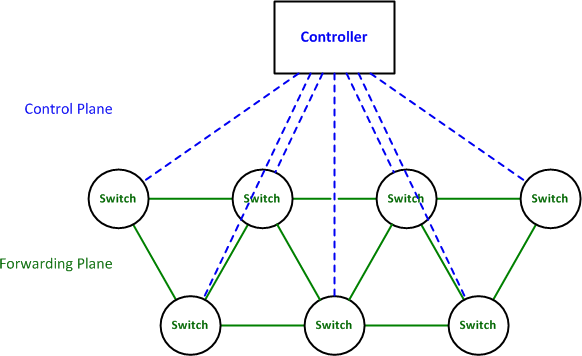
\includegraphics{imgs/SDN_controller.png}
	\caption{نمایی انتزاعی از معماری شبکه های نرم افزار محور}
	\label{fig1}
\end{figure}

\section{ویژگی های معماری \lr{SDN}}
\begin{enumerate}
	\item قابلیت برنامه ریزی مستفیم
	\item دینامیک بالا و تغییرات لحظه‌ای
	\item مدیریت متمرکز
	\item اختصاصی نبودن نرم افزار و سیستم عامل‌های شبکه
	\item مبتنی بر استاندارد‌های آزاد و عدم وابستگی به فروشنده تجهیز شبکه
\end{enumerate}

\section{اجزاء تشکیل دهنده معماری \lr{SDN}}

\begin{figure}
	\centering
	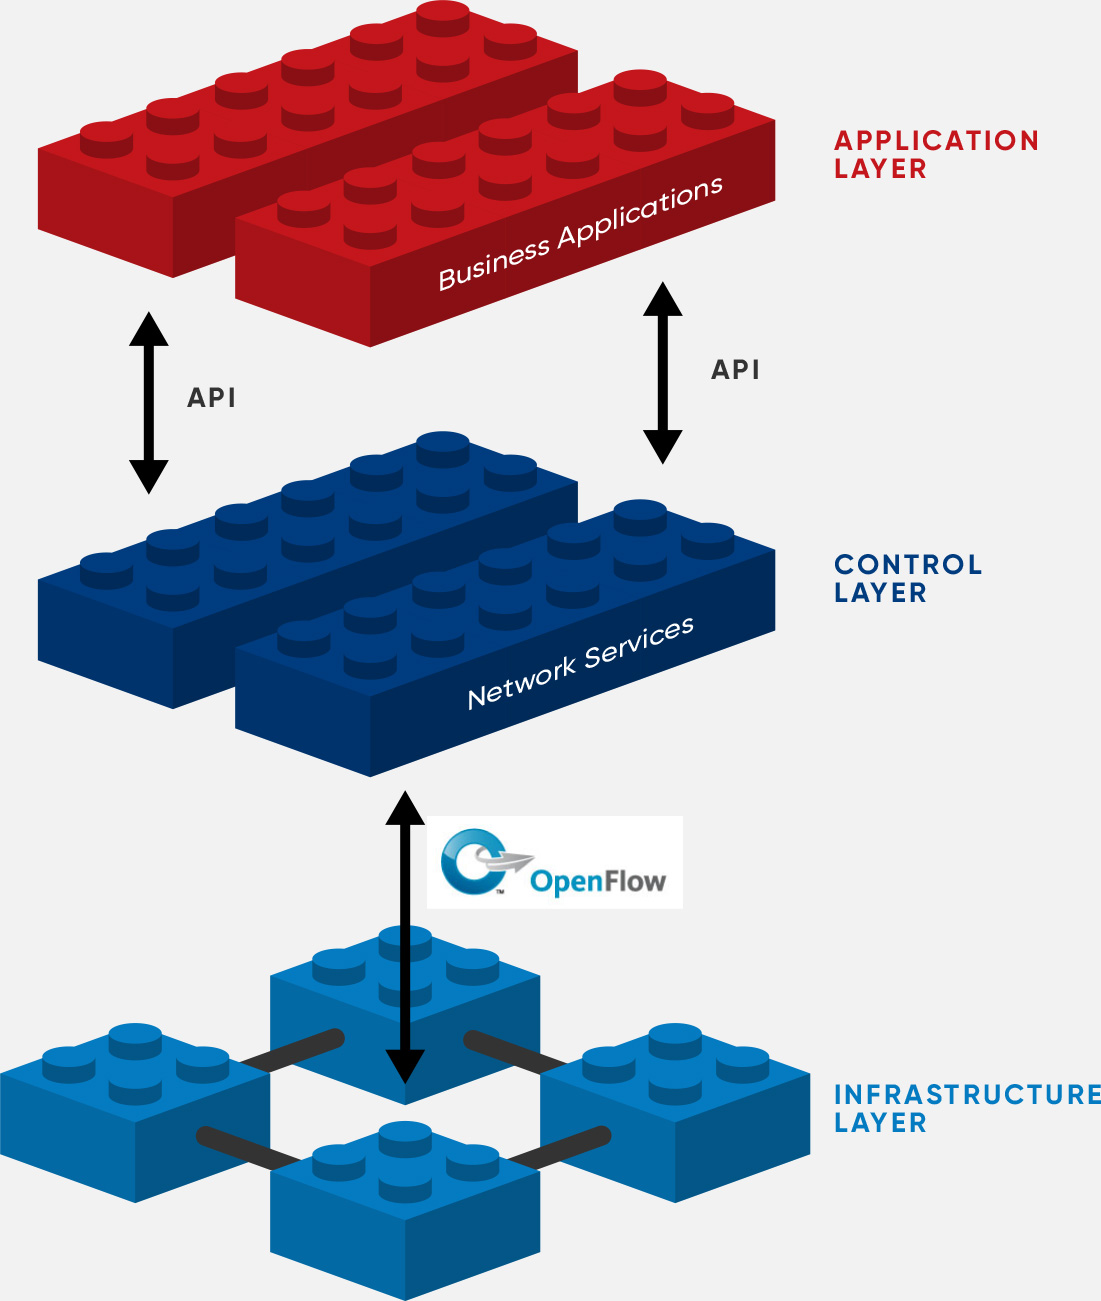
\includegraphics[scale=0.4]{imgs/sdn-architecture-img.jpg}
	\caption{نمایی از اجزاء تشکیل دهنده شبکه های مبتنی بر نرم‌افزار}
	\label{fig2}
\end{figure}